\section{Motivation: Hamiltonian mechanics}

% Now we've seen what symplectic manifolds are. Why are these interesting?

% One motivation comes from dynamical systems: there are many results about area-preserving maps in two dimensions (such as the Poincaré-Birkhoff theorem). In higher dimensions, there is a notion of volume-preserving maps, but the correct generalisation are symplectomorphisms. For instance, Poincaré-Birkhoff generalises into the Arnold conjecture. We'll see this again in a few moments.

% I'll tell you another reason, coming from classical physics.
% Consider a mechanical system. I've put two examples on my slide; the solar system and a double pendulum. They can be described by Newton's laws of mechanics, but perhaps slightly awkwardly: for instance, the pendulum's arm are rigid, this puts a constraint on the pendulum's evolution. We'd want our setup to encode such constraints. Hamiltonian mechanics is an equivalent way to describe Newton's axioms, but is more more elegant (and handles constraints nicely).
\begin{frame}
  \frametitle{Motivation: Hamiltonian mechanics}
  \pause
  \begin{minipage}{0.45\textwidth}
    \begin{figure}
      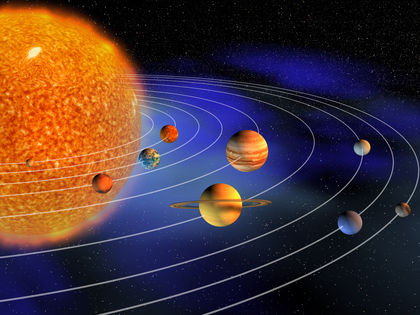
\includegraphics[width=5cm]{images/solar_system.jpg}\\
      The solar system (simplified).
%      \shrink{Source: \url{http://www.scienceclarified.com/photos/solar-system-2865.jpg}}
    \end{figure}
  \end{minipage}
  \hspace{1cm}
  \begin{minipage}{0.4\textwidth}
    \begin{figure}
      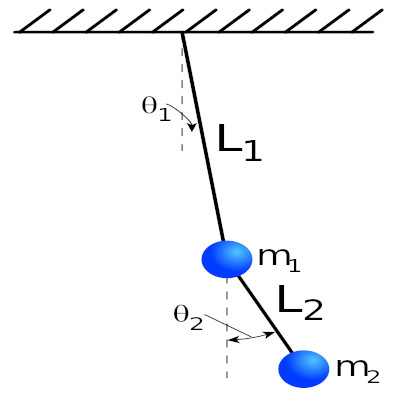
\includegraphics[height=3.5cm]{images/double_pendulum.jpg}\\
      A double pendulum.
%      \\\shrink{Source: By JabberWok, CC BY-SA 3.0, \url{https://commons.wikimedia.org/w/index.php?curid=1601029}}
    \end{figure}
  \end{minipage}
\end{frame}

% So, let's dive in. Let's derive the correct framework in the example of the n-body problem (such as the solar system).
\begin{frame}
  \frametitle{Hamiltonian systems: from Newton's to Hamilton's equations}
  \begin{itemize}
    % for k particles moving in R^3, we have 3 degrees of freedom per particles, hence 3k degrees of freedom overall. generally, a
    \item system of particles moving with n degrees of freedom %is described by a path in $R^n$,
    \[ q(t) = (q_1(t),\dots q_n(t)) \]
    \item \hide{gravitational interaction is conservative:}
    forces are derived from a \highlight{potential} $V(q)$ by $F(q)= -\grad V(q)$
    \item Newton's second law states $m_i \ddot{q_j} = - \frac{\partial V}{\partial q_j}$
    \hide{\item total energy
      \[ E := \mymark{blue}{\sum_{j=1}^n \frac{1}{2} m_j\, \dot{q}_j^2}{kinetic energy} + \mymark{red}{V(q)}{potential energy} \]
      is conserved: $\frac{\partial E}{\partial t}=0$}
    \pause

    % The Irish physicist Hamilton realised a better viewpoint for this.
    % His idea was to consider the momenta of the particles.
    \item Hamilton: consider momenta $p_j := m_j \dot{q_j}$
    \item total energy defines the Hamiltonian function
    \[ H\colon \R^{2n}\to\R,\quad (q,p)\mapsto \mymark{red}{\sum_{j=1}^n \frac{p_j^2}{2 m_j}}{kinetic energy} + \mymark{blue}{V(q)}{potential forces} \]
    \vspace{-\baselineskip}
    \item Newton's equations become \highlight{Hamilton's equations}
    \begin{equation*} \dot{q}_j = \frac{\partial H}{\partial p_j} \;\;\text{ and }\;\,\dot{p}_j = -\frac{\partial H}{\partial q_j}, \quad \text{ for }j=1,\dots n \tag{H}\end{equation*}
  \end{itemize}
\end{frame}

\begin{frame}
  \frametitle{Hamilton's equations on a manifold: symplectic manifolds}
  \begin{columns}
    \begin{column}{0.72\textwidth}
      \begin{itemize}
        % Hamilton's key insight was to treat the positions $q_j$ and momenta $p_j$ as independent variables, and to describe the motion of the system as a trajectory in $2n$-dimensional ``phase space''.
        \item key insight: regard $(q(t), p(t))$ as trajectory\\in \highlight{phase space} $\R^{2n} = T^\ast \R^n$

        % This is useful, since the phase space formalism also applies to the double pendulum! If we assume that both pendulums are rigid, we can describe the double pendulum by the two angles only, hence by two coordinates $q(t)=(q_1(t), q_2(t))$ in the torus. The torus is called the position or configuration space. The phase phase turns out to be the cotangent bundle of the position space.
        \item double pendulum: rigid arms \hide{and no friction} mean\\
        $q(t)=(q_1(t),q_2(t))\in \torus{2}$,\\phase space is cotangent bundle $T^\ast \torus{2}$
        % you may observe that \R^{2n}$ is the phase space of the position space \R^n above; this observation holds in general

        \item for systems with constraints, treat $(q,p)$\\as \highlight{local coordinates} of a point\\moving in a manifold
      \end{itemize}
    \end{column}
    \begin{column}{0.3\textwidth}
      \hspace{-8mm}\mbox{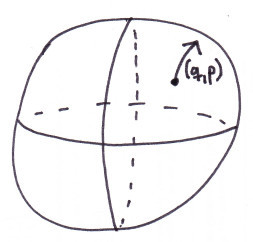
\includegraphics[width=4cm]{images/phase_space.jpg}}
    \end{column}
  \end{columns}

  \vspace{0.5\baselineskip}
  % issue: a system which satisfies Hamilton's equations for one choice of local coordinates need not satisfy it for all other choices. This motivates the following definition.
  \begin{block}{Fact}
    A smooth $2n$-dimensional manifold it is covered by coordinate charts $(q_1, p_1,\dots, q_n, p_n)$ such that for all smooth $H\colon M\to\R$, all coordinate changes preserve the form of (H) iff it is symplectic.
  \end{block}
  % Both R^2n and the cotangent bundle of any smooth manifold are symplectic.
\end{frame}

\begin{frame}
  \frametitle{Hamilton's equation in symplectic manifolds}
  \begin{definition}
    For $(M, \omega)$ symplectic, $H\colon \R\times M\to\R$ smooth, the \highlight{Hamiltonian vector field} $X_{H_t}$ of $H$ is defined by $\omega(X_{H_t}, \cdot) = -dH(t,\cdot)$.
    % an equality of $1$-forms; non-deg. of $\omega$ implies that $X_H$ is uniquely defined.
  \end{definition}
  \begin{block}{Exercise}
    Solutions $(q,p)$ of (H) are the integral curves of $X_H$.
    %A path $x(t)=(q(t),p(t))$ in $\R^{2n}$ satisfies Hamilton's equation iff $\dot{x}(t) = X_H(x(t))$. Thus: trajectories of a Hamiltonian system are integral curves = flow lines of the Hamiltonian vector field $X_H$!
  \end{block}
  % To summarize: symplectic manifolds are the natural setting for describing the evolution of Hamiltonian systems.
\end{frame}
